\chapter{原型系统与案例验证}

\section{原型系统构建}
% 原型系统架构用不用写?
\subsection{网络结构}
本系统部署在4台服务器,如表~\ref{tab:server-cfg}所示,其中“172.21.213.177”服务器是南师大地科院的刀片服务器上的虚拟机,CPU是E5-2630,10个核心,支持10个IBIS模型实例并行运行;“192.168.190.128”服务器是位于本地PC机的虚拟机上,CPU是i7-4770,4个核心,支持Biome-BGC和LPJ共4个实例并行运行;“172.21.212.58”服务器也是南师大地科院的刀片服务器上的虚拟机,硬盘大小200GB,支持大容量数据快速存取;“223.2.35.73”服务器位于本地PC机,CPU是i7-4770,8个核心。这些服务器都位于同一个局域网下,保证了数据传输速度。

\begin{table}[H]
    \centering
    \caption{服务器部署配置}
    \label{tab:server-cfg}
    \begin{threeparttable}
        \begin{tabular}{lllllll}
            \Xhline{1.5pt}
            层级 & 地址 & 端口 & 部署的微服务 \\
            \Xhline{1pt}
            \multirow{3}{*}{模型计算层} & 172.21.213.177 & 6868 & IBIS服务 \\
            % \cline{2-4}
            & \multirow{2}{*}{192.168.190.128} & \multirow{2}{*}{6868} & Biome-BGC服务 \\
            % \cline{4-4}
            &&& LPJ服务 \\
            \hline
            \multirow{4}{*}{数据管理层} & \multirow{4}{*}{172.21.212.58} & \multirow{3}{*}{8786} & 数据上传服务 \\
            % \cline{4-4}
            &&& 数据下载服务 \\
            % \cline{4-4}
            &&& 数据重构服务 \\
            % \cline{3-4}
            && 8787 & WMS WFS WCS \\
            \hline
            模型对比层 & 223.2.35.73 & 9999 & 对比服务 \\
            \Xhline{1.5pt}
        \end{tabular}
    \end{threeparttable}
\end{table}

\subsection{微服务容器}
服务容器作为服务的承载工具,它本身并不处理非常复杂的计算逻辑,而是将CPU密集型操作交给它所容纳的服务,所以服务容器是IO密集型的程序,他需要处理高并发的HTTP请求。Node.js作为异步编程的代表,天生适合这种场景,所以本文选择Node.js作为后台服务容器开发语言,使用MongoDB管理数据。由于Node.js的单线程特性,它本身并不稳定,所以使用PM2进行单台服务节点上Node.js应用的负载均衡。

\begin{figure}[!htbp]
    \centering
    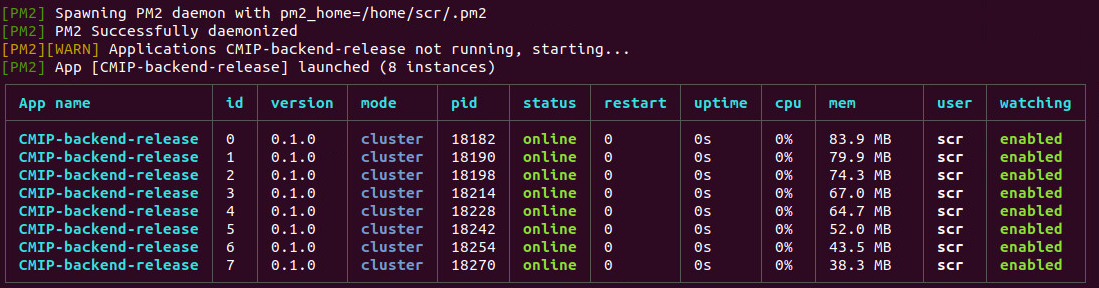
\includegraphics[width=1\textwidth]{PM2}
    \caption{PM2负载均衡管理}
    \label{fig:ms-step}
\end{figure}

微服务容器作为面向管理员的后台管理工具,数据管理容器、模型计算容器和模型对比容器都具有很多通用的功能,如图~\ref{fig:service-container-common-fn}所示,微服务容器可以对服务进行管理,包括发布、注销、实例管理等,此外,还可以对服务器性能进行监控。

\begin{figure}[!htbp]
    \centering
    \subcaptionbox{服务列表、重新发布、注销\label{fig:service-publish-removal}}{
\includegraphics[width=.45\textwidth]{ms-step}}
    \hfill
    \subcaptionbox{服务上传部署发布\label{fig:service-deploy}}{
\includegraphics[width=.45\textwidth]{ms-step}} \\
    \subcaptionbox{服务实例管理\label{fig:insitance-manage}}{
\includegraphics[width=.45\textwidth]{ms-step}}
    \hfill
    \subcaptionbox{服务器性能监测\label{fig:monitor}}{
\includegraphics[width=.45\textwidth]{ms-step}}
    \caption{微服务容器通用功能}
    \label{fig:service-container-common-fn}
\end{figure}

除了通用功能,数据管理容器通过Nginx的消息中转还支持使用GeoServer发布WMS、WFS、WCS服务(图~\ref{fig:geoserver}),模型对比容器支持对计算节点进行管理(图~\ref{fig:api-gateway-children})。

\begin{figure}[!htbp]
    \centering
    
\includegraphics[width=1\textwidth]{ms-step}
    \caption{GeoServer发布数据服务}
    \label{fig:geoserver}
\end{figure}

\begin{figure}[!htbp]
    \centering
    
\includegraphics[width=1\textwidth]{ms-step}
    \caption{API网关(对比服务容器)上注册的子节点}
    \label{fig:api-gateway-children}
\end{figure}

\subsection{陆地生态系统碳循环模型对比门户网站}
面向开放式模型计算和对比的需求,本文构建了一个门户网站,作为对比方案和对比结果共享的入口。一方面可以将对比过程和结果公开化,降低碳循环模型的使用难度,另一方面可以激励模式组的模型通过封装加入进来,促进碳循环研究的发展。门户网站的主要功能模块设计为如图\ref{fig:system-module},功能模块分为资源模块、对比业务模块、结果展示模块和用户管理模块,其中资源模块包括模型资源和数据资源;对比业务模块则对应于对比话题、对比方案和对比任务;结果展示模块基于所有对比任务的执行结果,将对比结果展示出去;用户模块包括用户的个人资源管理。门户网站的登录、注册和首页如图~\ref{fig:portal-index}所示。

\begin{figure}[!htbp]
    \centering
    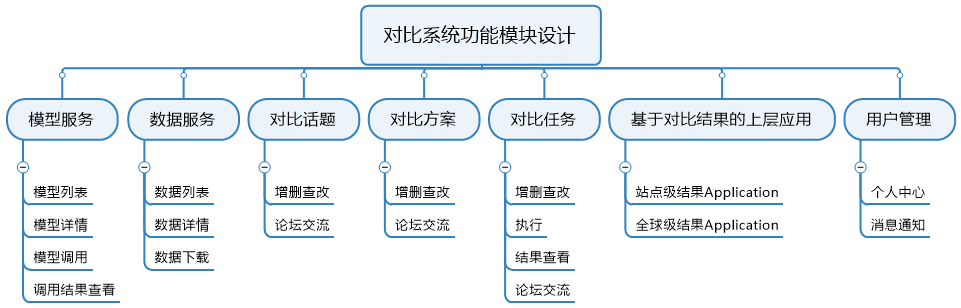
\includegraphics[width=1\textwidth]{system-module}
    \caption{对比系统功能模块设计}
    \label{fig:system-module}
\end{figure}

\begin{figure}[!htbp]
    \centering
    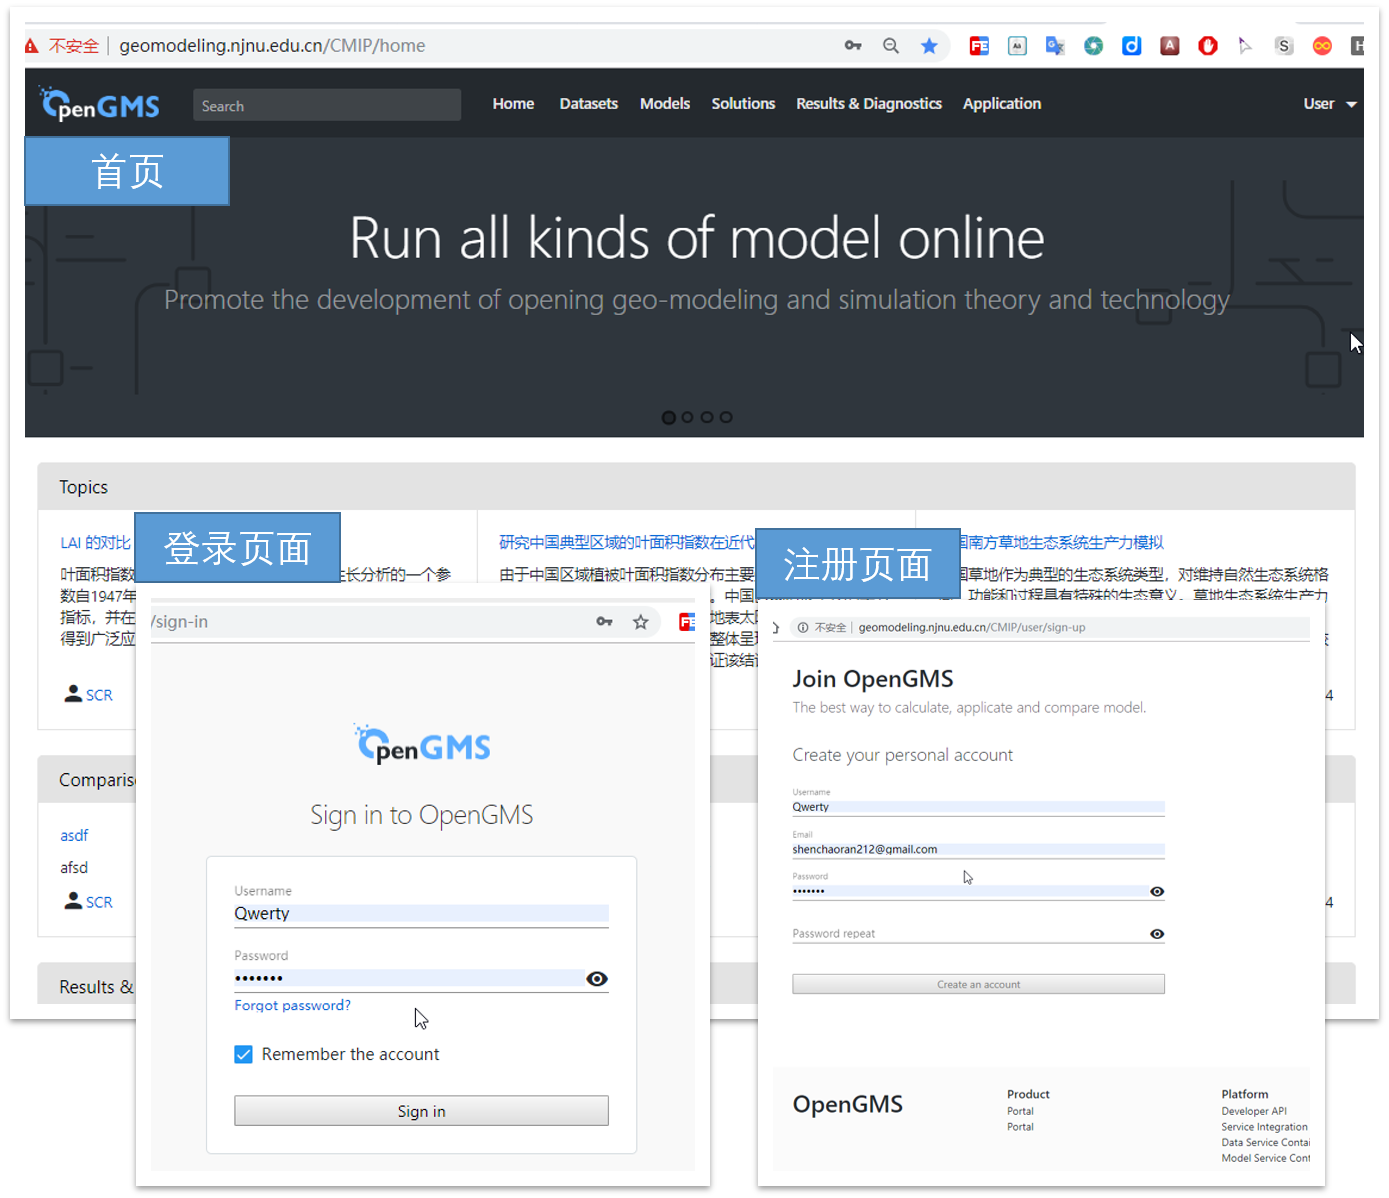
\includegraphics[width=.7\textwidth]{portal-index}
    \caption{门户网站首页和注册登录页面}
    \label{fig:portal-index}
\end{figure}

\begin{figure}[!htbp]
    \centering
    \subcaptionbox{模型资源和数据资源列表\label{fig:ms-data-resource}}{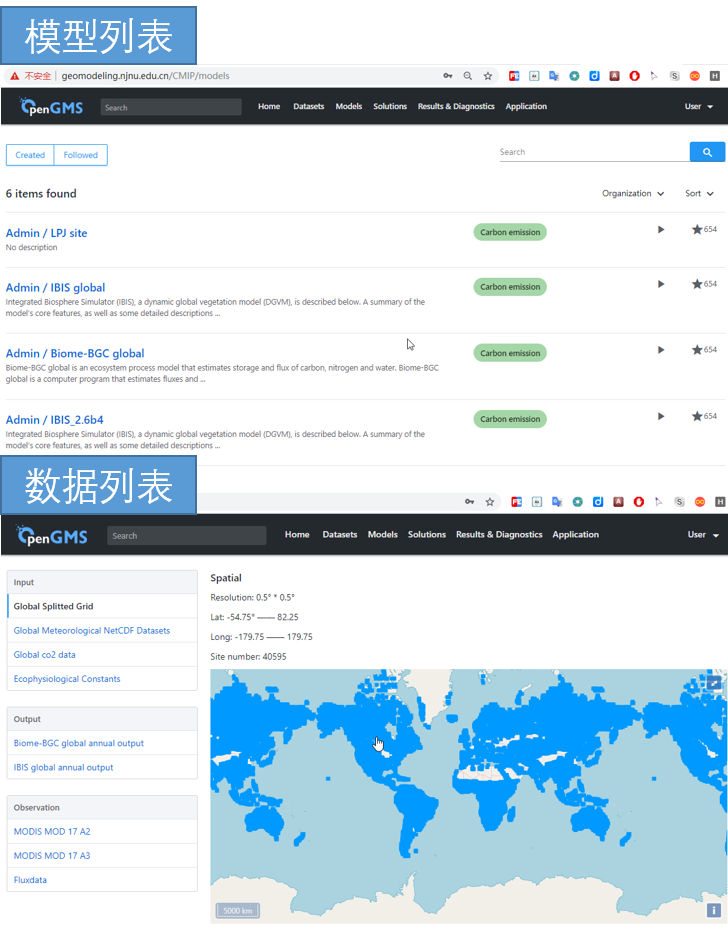
\includegraphics[width=.5\textwidth]{ms-data-resource}}
    \hfill
    \subcaptionbox{模型服务调用\label{fig:ms-invoke}}{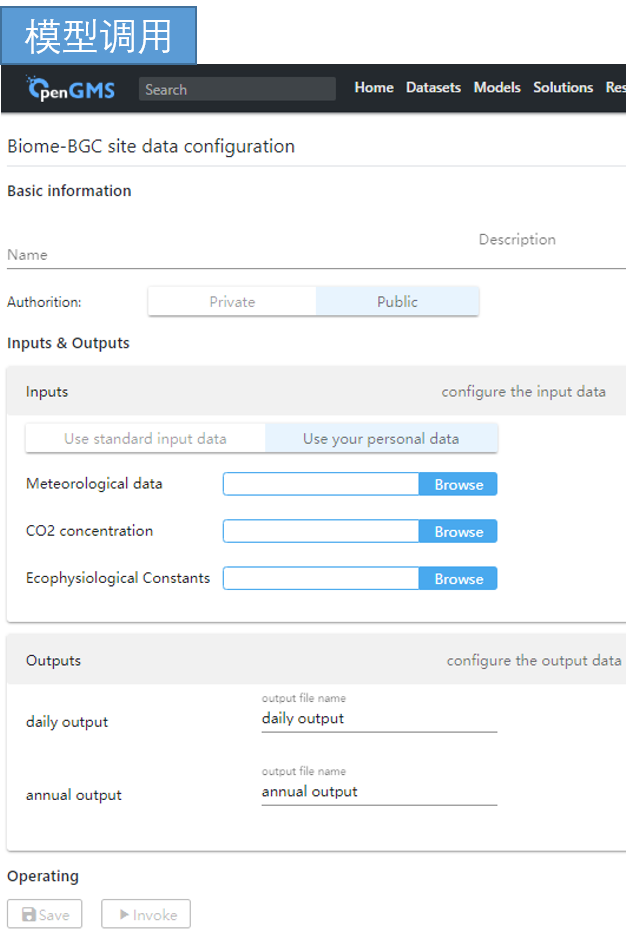
\includegraphics[width=.43\textwidth]{ms-invoke}}
    \caption{门户网站模型和数据资源}
    \label{fig:portal-resource}
\end{figure}

\begin{figure}[!htbp]
    \centering
    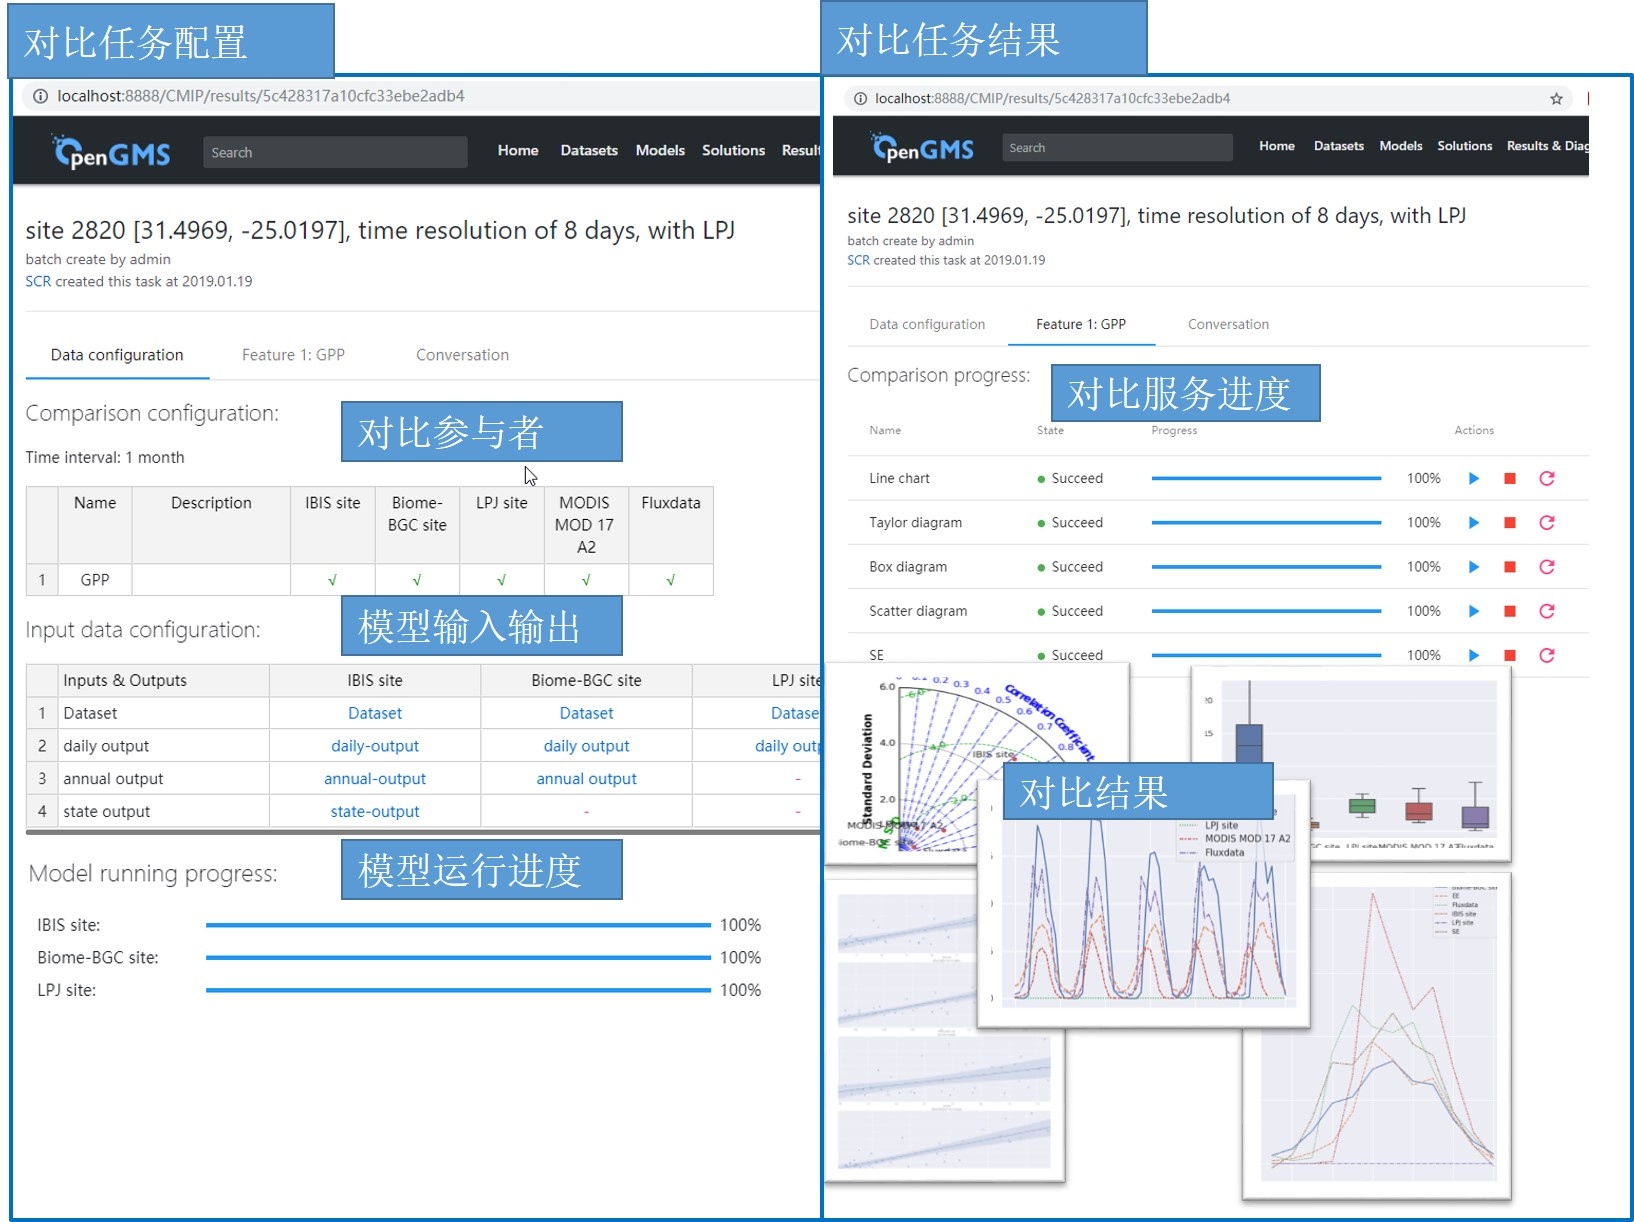
\includegraphics[width=1\textwidth]{task-cfg-result}
    \caption{对比任务配项和结果}
    \label{fig:task-cfg-result}
\end{figure}

\begin{figure}[!htbp]
    \centering
    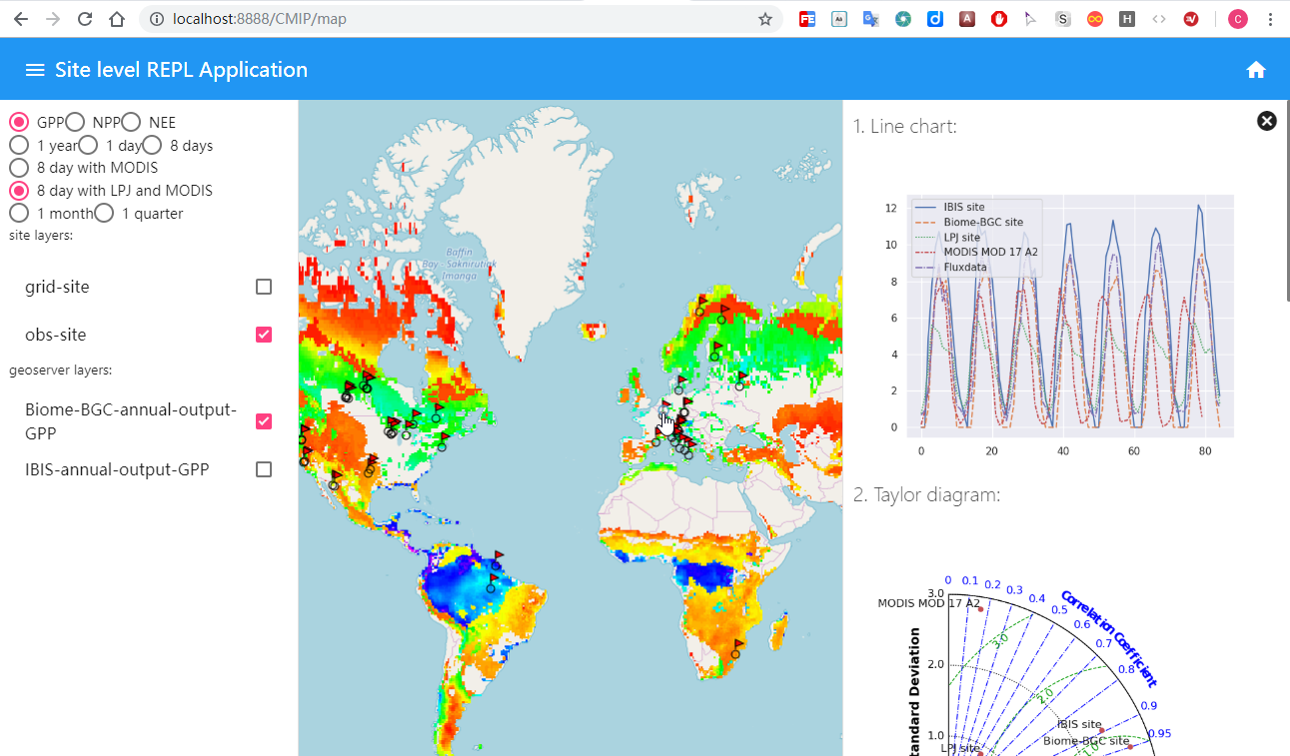
\includegraphics[width=.8\textwidth]{site-REPL}
    \caption{站点级对比结果查询应用}
    \label{fig:site-REPL}
\end{figure}

\section{实验案例}
\subsection{模型资源和数据资源}
\subsection{对比方案}
\subsection{对比结果}
% 时间变化
% 空间变化
% 历史变化
% 未来预估